\documentclass{article}[18pt]
\ProvidesPackage{format}
%Page setup
\usepackage[utf8]{inputenc}
\usepackage[margin=0.7in]{geometry}
\usepackage{parselines} 
\usepackage[english]{babel}
\usepackage{fancyhdr}
\usepackage{titlesec}
\hyphenpenalty=10000

\pagestyle{fancy}
\fancyhf{}
\rhead{Sam Robbins}
\rfoot{Page \thepage}

%Characters
\usepackage{amsmath}
\usepackage{amssymb}
\usepackage{gensymb}
\newcommand{\R}{\mathbb{R}}

%Diagrams
\usepackage{pgfplots}
\usepackage{graphicx}
\usepackage{tabularx}
\usepackage{relsize}
\pgfplotsset{width=10cm,compat=1.9}
\usepackage{float}

%Length Setting
\titlespacing\section{0pt}{14pt plus 4pt minus 2pt}{0pt plus 2pt minus 2pt}
\newlength\tindent
\setlength{\tindent}{\parindent}
\setlength{\parindent}{0pt}
\renewcommand{\indent}{\hspace*{\tindent}}

%Programming Font
\usepackage{courier}
\usepackage{listings}
\usepackage{pxfonts}

%Lists
\usepackage{enumerate}
\usepackage{enumitem}

% Networks Macro
\usepackage{tikz}


% Commands for files converted using pandoc
\providecommand{\tightlist}{%
	\setlength{\itemsep}{0pt}\setlength{\parskip}{0pt}}
\usepackage{hyperref}

% Get nice commands for floor and ceil
\usepackage{mathtools}
\DeclarePairedDelimiter{\ceil}{\lceil}{\rceil}
\DeclarePairedDelimiter{\floor}{\lfloor}{\rfloor}

% Allow itemize to go up to 20 levels deep (just change the number if you need more you madman)
\usepackage{enumitem}
\setlistdepth{20}
\renewlist{itemize}{itemize}{20}

% initially, use dots for all levels
\setlist[itemize]{label=$\cdot$}

% customize the first 3 levels
\setlist[itemize,1]{label=\textbullet}
\setlist[itemize,2]{label=--}
\setlist[itemize,3]{label=*}

% Definition and Important Stuff
% Important stuff
\usepackage[framemethod=TikZ]{mdframed}

\newcounter{theo}[section]\setcounter{theo}{0}
\renewcommand{\thetheo}{\arabic{section}.\arabic{theo}}
\newenvironment{important}[1][]{%
	\refstepcounter{theo}%
	\ifstrempty{#1}%
	{\mdfsetup{%
			frametitle={%
				\tikz[baseline=(current bounding box.east),outer sep=0pt]
				\node[anchor=east,rectangle,fill=red!50]
				{\strut Important};}}
	}%
	{\mdfsetup{%
			frametitle={%
				\tikz[baseline=(current bounding box.east),outer sep=0pt]
				\node[anchor=east,rectangle,fill=red!50]
				{\strut Important:~#1};}}%
	}%
	\mdfsetup{innertopmargin=10pt,linecolor=red!50,%
		linewidth=2pt,topline=true,%
		frametitleaboveskip=\dimexpr-\ht\strutbox\relax
	}
	\begin{mdframed}[]\relax%
		\centering
		}{\end{mdframed}}



\newcounter{lem}[section]\setcounter{lem}{0}
\renewcommand{\thelem}{\arabic{section}.\arabic{lem}}
\newenvironment{defin}[1][]{%
	\refstepcounter{lem}%
	\ifstrempty{#1}%
	{\mdfsetup{%
			frametitle={%
				\tikz[baseline=(current bounding box.east),outer sep=0pt]
				\node[anchor=east,rectangle,fill=blue!20]
				{\strut Definition};}}
	}%
	{\mdfsetup{%
			frametitle={%
				\tikz[baseline=(current bounding box.east),outer sep=0pt]
				\node[anchor=east,rectangle,fill=blue!20]
				{\strut Definition:~#1};}}%
	}%
	\mdfsetup{innertopmargin=10pt,linecolor=blue!20,%
		linewidth=2pt,topline=true,%
		frametitleaboveskip=\dimexpr-\ht\strutbox\relax
	}
	\begin{mdframed}[]\relax%
		\centering
		}{\end{mdframed}}
\lhead{Software Methodologies - Image Processing}


\begin{document}
\begin{center}
\underline{\huge Lecture 1}
\end{center}
\begin{defin}[Assistive imaging]
Enhancement, Restoration, representation or transformation of visual data to aid in visualisation and interpretation by humans or as pre-processing step for computer vision	
\end{defin}
\begin{defin}[Computer Vision]
	Automatic interpretation of visual data using computers without human intervention	
\end{defin}
\begin{defin}[Image]
A multidimensional signal, commonly containing visual information (in general regularly sampled)	
\end{defin}

\textbf{Pixel} - Picture Element\\
\\
\textbf{Spatial Resolution}: $X\times Y$ (horizontal by vertical) dimensions of the image\\
\\
Direct computation gives the number of pixels used to cover the visual space captured by the image relates to the sampling of the image signal\\
\\
\textbf{Colour Resolution} - The dimension of the colour space - known as quantization\\
\\
\textbf{Temporal Resolution}: In continuous capture systems (e.g. video) the number of images captured in a given time period
\section{Representational Requirements}
Scenes have to be sampled (spatially, temporally) and quantized in what is essentially an analogue to digital conversion.\\
The sampling must be high enough to preserve useful information in the image. Quantisation must avoid aliasing
\section{Aliasing}
As resolution is limited, there is aliasing effects.
\begin{center}
	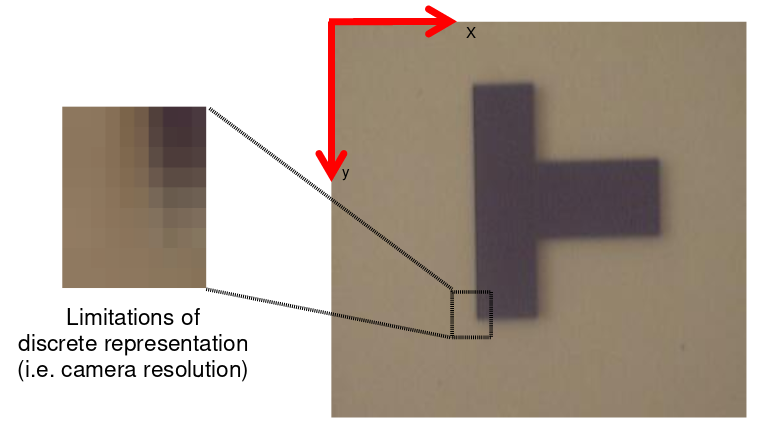
\includegraphics[scale=0.7]{Aliasing}
\end{center}
An analogue signal will always suffer some form of aliasing in the digitisation process - at some level
\begin{center}
	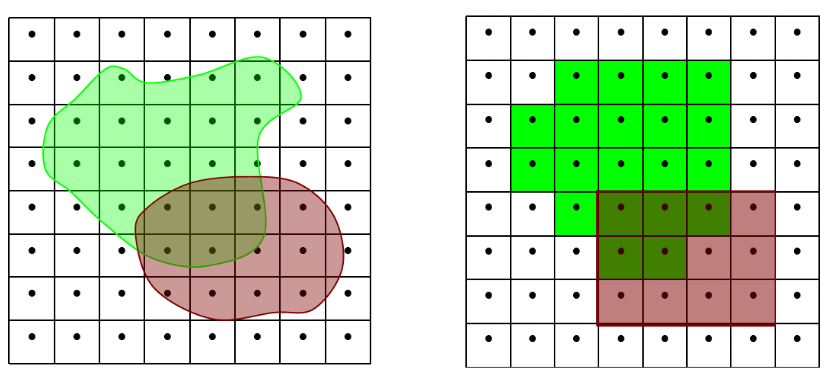
\includegraphics[scale=0.7]{Aliasing1}
\end{center}
Aliasing effects both the connectivity and topological measurement image features - noise is introduced. Image processing algorithms must be able to cope with the problems arising from this form of sampling noise
\section{Colour (or intensity) quantization}
At each pixel there is a voltage reading on the image sensor that relates to the amount and wavelength of light received.\\
It is discretised into a number of bins representing a level of intensity.
\section{Image colour channels}
Red, green abd blue light intensity for each (x,y) pixel gives an \{r,g,b\} integer vector.\\
\\
Colour image = 3-channel image (x,y,i) for i=\{0,1,2\}\\
\\
Greyscale = 1 channel
\section{Pixel co-ordinates}
Greyscale images: image(x,y) = value\\
Colour images: image(x,y) = (r,g,b)\\
Pixel location: (x,y) position in the column by row coordinate system.\\
\\
Positive co-ordinate system: origin = top left\\
\\
Origin is not universal: OpenCV uses top left and:
\begin{center}
	column (c) = x co-ordinate\\
	row (r) = y co-ordinate
\end{center}
\section{What do pixel values actually represent in image data?}
\textbf{Intensity/colour}: Wavelength or intensity of light\\
\textbf{Infra-red}: Infra-red electromagnetic intensity
\begin{itemize}
	\item Near and far infra-red are different wavelengths
	\item Visualisation may require colour mapping
\end{itemize}
\textbf{Medical CT/ MRI} - Pixel values are proportional to the absorption characteristics of tissue in relation to a signal sent through the body
\begin{itemize}
	\item Segmentation
	\item Visualisation of volumetric data
\end{itemize}
\textbf{Radar} - Pixel values are proportional to target distance from the sensor and reflectivity
\begin{itemize}
	\item Calibrating values correspond to distance
	\item Noise
\end{itemize}
\textbf{Depth/distance} - Pixel values encode distance of object/surface from sensor
\begin{itemize}
	\item Explicit 3D information rather than just a 2D projection, but partial only view of the captured 3D object
\end{itemize}
\textbf{Scientific} - Pixel values encode measurements from a given sensor
\begin{itemize}
	\item Representation: positive and negative floating point image values
	\item Visualisation: colour mapping/negative value scaling
\end{itemize}




\end{document}